
\chapter{Applying the model}
\section{Non-dimensionalising the equations of motion}
When the number of cells is fixed at $N \geq 1$ we have the following equations of motion,
which consist of the equations of motion for the biomass node network (governed by forces) and 
the reaction diffusion PDE of the nutrient field. Let the spring connectivity
be given by the matrix $A_{ij}$ where $i$ and $j$ index over the number of cells and $A_{ij}$
is $1$ if node $i$ is connected to node $j$ by an edge and $0$ otherwise.
\begin{equation*}
    \frac{d \vb{x}_i }{dt} = 
    \frac{1}{\eta} \left[\sum_{j = 1, j \neq i}^N   \left(A_{ij} \vb{F}_{\textrm{spring},ij} + 
     \vb{F}_{\textrm{contact},ij} \right) +\vb{F}_{\textrm{chemo},i}  \right] ,
    \ \textrm{for} \ i = 1, ... , N.
\end{equation*}
\begin{equation*}
    \pdv{c}{t} = D \left(\pdv[2]{c}{x} + \pdv[2]{c}{y} \right) - r c b,
\end{equation*}
where the biomass field $b$ is given by 
\begin{equation*}
b(x,y,t) = \begin{cases}
            -\beta g(x,y,t), & \ \textrm{if} \ g(x,y,t) \leq 0, \\
                0, &    \ \textrm{otherwise},
           \end{cases}
\end{equation*}
where the field $g(x,y,t) =\textrm{smoothmin}(f_1(x,y,t), ...,f_N(x,y,t) )$ where 
$f_e(x,y,t)$ is the signed distance field for the $e$-th cell ($e$ indexes over the egdes).
Here the spring force is given by 
\begin{equation}
    \vb{F}_{\textrm{spring},ij} = -K\left( ||\vb{x}_i - \vb{x}_j|| - L_0\right) \frac{\vb{x}_i - \vb{x}_j}{||\vb{x}_i - \vb{x}_j||},
\end{equation}
the contact force is given by 
\begin{equation}
    \vb{F}_{\textrm{contact},ij} = F H(R - ||\vb{x}_i - \vb{x}_j||) \frac{\vb{x}_i - \vb{x}_j}{||\vb{x}_i - \vb{x}_j||} ,
\end{equation}
and the force of chemotaxis is given by 
\begin{equation*}
    \vb{F}_{\textrm{chemo},i} = \gamma \nabla c (\vb{x}_i, t).
\end{equation*}
The constants are defined as follows. 
\begin{itemize}
    \item $\eta$ is the viscous damping in the overdamped regime.
    \item $K$ is the spring constant which applies to each spring in the colony.
    \item $D$ is the nutrient diffusion constant.
    \item $\beta$ converts from a signed distance field to a microscopic biomass density.
    \item $r$ is the rate at which nutrient is metabolised by the biomass.
    \item $L_0$ is the major diameter of the elliptical cell.
    \item $F$ is the magnitude of the contact force between cells.
    \item $R$ is the activation radius of the contact force.
    \item $\gamma$ is the magnitude of the chemotactic force.
    \item $k$ is the smoothness parameter for the smoothmin.
\end{itemize}
We make a subsitution of the following dimensionless (hatted) parameters,
\begin{equation*}
    \vb{x}_i = L\hat{\vb{x}}_i,,
\end{equation*}
\begin{equation*}
    t = T\hat{t}
\end{equation*}
\begin{equation*}
    c = c_0 \hat{c},
\end{equation*}
\begin{equation*}
    b = \frac{M}{L^2}\hat{b},
\end{equation*}
\begin{equation*}
    \eta = E \hat{\eta},
\end{equation*}
\begin{equation*}
    K = \kappa \hat{K},
\end{equation*}
\begin{equation*}
    D = \frac{L^2}{T} \hat{D},
\end{equation*}
\begin{equation*}
    \beta = B \hat{\beta},
\end{equation*}
\begin{equation*}
    r = \frac{L^2}{M T} \hat{r},
\end{equation*}
\begin{equation*}
    L_0 = L \hat{L}_0,
\end{equation*}
\begin{equation*}
    F = \phi \hat{F},
\end{equation*}
\begin{equation*}
    R = L \hat{R},
\end{equation*}
\begin{equation*}
    \gamma = \Gamma \hat{\gamma},
\end{equation*}
\begin{equation*}
    k = L \hat{k},
\end{equation*}in
into the equations of motion to derive dimensionless equations. The reaction-diffusion equation 
if given by 
\begin{equation*}
    \frac{c_0}{T}\pdv{\hat{c}}{\hat{t}} = \frac{L^2}{T} \hat{D} \frac{c_0}{L^2} \left(\pdv[2]{\hat{c}}{\hat{x}} + \pdv[2]{\hat{c}}{\hat{y}} \right) -
     \frac{L^2}{M T} \hat{r} c_0 \hat{c} \frac{M}{L^2} \hat{b},
\end{equation*}
which simplifies to 
\begin{equation*}
    \pdv{\hat{c}}{\hat{t}} =  \hat{D} \left(\pdv[2]{\hat{c}}{\hat{x}} + \pdv[2]{\hat{c}}{\hat{y}} \right) -
      \hat{r} \hat{c} \hat{b}.
\end{equation*}
The equation of motion for the position of the $i$-th node is 
\begin{equation*}
\begin{split}
    \frac{d \vb{x}_i}{dt} &= 
    \frac{1}{ \eta}\sum_{j = 1, j \neq i}^N   \left[ - A_{ij} K\left( ||\vb{x}_i - \vb{x}_j|| - L_0\right) \frac{\vb{x}_i - \vb{x}_j}{||\vb{x}_i - \vb{x}_j||} \right]\\
     &+ \frac{1}{ \eta}\sum_{j = 1, j \neq i}^N \left[F H(R - ||\vb{x}_i - \vb{x}_j||) \frac{\vb{x}_i - \vb{x}_j}{||\vb{x}_i - \vb{x}_j||}     \right]\\ 
     &+ \frac{1}{\eta} \gamma \nabla c (\vb{x}_i, t),
\end{split}
\end{equation*}
Substituting the non-dimesnionalised variables, we arrive at
\begin{equation*}
    \begin{split}
        \frac{L}{T}\frac{d \hat{\vb{x}}_i}{d \hat{t}} &= 
        \frac{1}{E  \hat{\eta}}\sum_{j = 1, j \neq i}^N   \left[ - A_{ij} \kappa \hat{K}\left( L||\hat{\vb{x}}_i - \hat{\vb{x}}_j|| - L \hat{L}_0\right) \frac{\hat{\vb{x}}_i - \hat{\vb{x}}_j}{||\hat{\vb{x}}_i - \hat{\vb{x}}_j||} \right]\\
         &+ \frac{1}{E  \hat{\eta}}\sum_{j = 1, j \neq i}^N \left[\phi\hat{F} H(\hat{R} - ||\hat{\vb{x}}_i - \hat{\vb{x}}_j||) \frac{\hat{\vb{x}}_i - \hat{\vb{x}}_j}{||\hat{\vb{x}}_i - \hat{\vb{x}}_j||}     \right]\\ 
         &+ \frac{1}{E  \hat{\eta}}\Gamma \hat{\gamma} \frac{c_0}{L} \hat{\nabla}  \hat{c} (\hat{\vb{x}}_i, \hat{t}),
    \end{split}
\end{equation*}
which simplifies to 
\begin{equation*}
    \begin{split}
        \frac{d \hat{\vb{x}}_i}{d \hat{t}} &= 
        \left(\frac{T \kappa}{E }\right) \frac{\hat{K}}{\hat{\eta}}\sum_{j = 1, j \neq i}^N   \left[ - A_{ij} \left(||\hat{\vb{x}}_i - \hat{\vb{x}}_j|| - \hat{L}_0\right) \frac{\hat{\vb{x}}_i - \hat{\vb{x}}_j}{||\hat{\vb{x}}_i - \hat{\vb{x}}_j||} \right]\\
         &+ \left(\frac{T \phi}{L E}\right)\frac{\hat{F}}{\hat{\eta}}\sum_{j = 1, j \neq i}^N \left[H(\hat{R} - ||\hat{\vb{x}}_i - \hat{\vb{x}}_j||) \frac{\hat{\vb{x}}_i - \hat{\vb{x}}_j}{||\hat{\vb{x}}_i - \hat{\vb{x}}_j||}     \right]\\ 
         &+ \left(\frac{T c_0 \Gamma}{ E L^2} \right) \frac{\hat{\gamma}}{ \hat{\eta}}   \hat{\nabla}  \hat{c} (\hat{\vb{x}}_i, \hat{t}).
    \end{split}
\end{equation*}
Since the mass of a yeast cell is roughly known to be on the order of $50$ pico-grams, we
introduce the mass constant $M$. Now the units of the viscocity constant $E$ are $[E] = \frac{[F]}{[v]}$
where $[F]$ and $[v]$ are the units of force and velocity, respectively. So this motivates us to 
try 
\begin{equation*}
    E = \frac{M}{T}.
\end{equation*}
We will also note the units of $\phi$ are force so
\begin{equation*}
    \phi = \frac{ML}{T^2},
\end{equation*}
and that the units of $\kappa$ are force per length so
\begin{equation*}
    \kappa = \frac{M}{T^2}.
\end{equation*}
Also it is necessary to introduce a characteristic area density for the nutrient field,
call it $\sigma \frac{M}{L^2}$, which has units of mass per length squared. We may aswell say that 
\begin{equation}
    c_0 = \sigma \frac{M}{L^2}.
\end{equation}
Note that the $\sigma$ acts as a multiplicative factor because the characteristic mass of yeast
and nutrient may be different. Indeed,
\begin{equation}
     \sigma = \frac{M_c}{M}.
\end{equation}
where $M_c$ is a characteristic mass unit for a glucose mixture. Based on dimesnional 
analysis alone, we make the choice 
\begin{equation}
    \Gamma = \frac{1}{\sigma} \frac{L^4}{T^2}.
\end{equation}
After all this, the equation for the node positions simplify to 
\begin{equation*}
    \begin{split}
        \frac{d \hat{\vb{x}}_i}{d \hat{t}} &= 
        \lambda_1 \sum_{j = 1, j \neq i}^N   \left[ - A_{ij} \left(||\hat{\vb{x}}_i - \hat{\vb{x}}_j|| - \hat{L}_0\right) \frac{\hat{\vb{x}}_i - \hat{\vb{x}}_j}{||\hat{\vb{x}}_i - \hat{\vb{x}}_j||} \right]\\
         &+ \lambda_2\sum_{j = 1, j \neq i}^N \left[H(\hat{R} - ||\hat{\vb{x}}_i - \hat{\vb{x}}_j||) \frac{\hat{\vb{x}}_i - \hat{\vb{x}}_j}{||\hat{\vb{x}}_i - \hat{\vb{x}}_j||}     \right]\\ 
         &+ \lambda_3  \hat{\nabla}  \hat{c} (\hat{\vb{x}}_i, \hat{t}).
    \end{split}
\end{equation*}
where $\lambda_1 = \frac{\hat{K}}{\hat{\eta}}$, $\lambda_2 = \frac{\hat{F}}{\hat{\eta}}$ and 
$\lambda_3 = \frac{\hat{\gamma}}{\hat{\eta}}$. We also use the same numbering convention for the PDE,
obtaining
\begin{equation*}
    \pdv{\hat{c}}{\hat{t}} =  \lambda_4 \left(\pdv[2]{\hat{c}}{\hat{x}} + \pdv[2]{\hat{c}}{\hat{y}} \right) -
      \lambda_5 \hat{c} \hat{b},
\end{equation*}
where $\lambda_4 = \hat{D}$ and $\lambda_5 = \hat{r}$. Finally, the equation for the biomass 
field is given by 
\begin{equation*}
    \frac{1}{L^2}\hat{b} = \begin{cases}
                -B \hat{\beta} L \hat{g}(\hat{x},\hat{x},\hat{t}), & \ \textrm{if} \ \hat{g}(\hat{x},\hat{x},\hat{t}) \leq 0, \\
                    0, &    \ \textrm{otherwise},
               \end{cases}
\end{equation*}
which motives the choice
\begin{equation*}
    B = \frac{1}{L^3},
\end{equation*}
which derives 
\begin{equation*}
    \hat{b} = \begin{cases}
                - \hat{\beta} \hat{g}(\hat{x},\hat{x},\hat{t}), & \ \textrm{if} \ \hat{g}(\hat{x},\hat{x},\hat{t}) \leq 0, \\
                    0, &    \ \textrm{otherwise}.
               \end{cases}
\end{equation*}
We let $\lambda_6 = \hat{\beta}$.
\\
\\

There are a few more parameters to include relating to the addition of new cells over time.
The average time taken to add a new cell into the simulation will be given by $\lambda_7$.
In other words, the problem now is to to try and choose the seven model values
\begin{equation*}
    \vb{\lambda} = (\lambda_1, \lambda_2, ..., \lambda_7), 
\end{equation*}
to produce a simulation that looks ``close'' to experimental data. 

\section{Introducing a potential function}
The equation of motion for the nodes can be rewritten in terms of a potential
if we first approximate the contact force by a smooth step function.
Let the Heaviside function be replaced by 
\begin{equation*}
    H(\hat{R} - ||\hat{\vb{x}}_i - \hat{\vb{x}}_j||) = \frac{1}{2} + \frac{1}{2} \tanh\left( \frac{\hat{R} - ||\hat{\vb{x}}_i - \hat{\vb{x}}_j||}{\hat{k}}\right)
\end{equation*}
where $\hat{k}$ is the (dimensionless) smoothness parameter (same as for the SDFs). The same parameter is chosen
to minimise the number of variables. We can now introduce the potential function 
\begin{equation*}
    \begin{split}
        \hat{\Phi}(\hat{\vb{x}}_i, \hat{t}) &= 
        -\lambda_1 \sum_{j = 1, j \neq i}^N   \left[ A_{ij} \frac{1}{2}\left(||\hat{\vb{x}}_i - \hat{\vb{x}}_j|| - \hat{L}_0\right)^2  \right]\\
         &- \lambda_2\sum_{j = 1, j \neq i}^N \frac{1}{2}\left[||\hat{\vb{x}}_i - \hat{\vb{x}}_j|| - 
            \hat{k} \log(\cosh\left( \frac{\hat{R} - ||\hat{\vb{x}}_i - \hat{\vb{x}}_j||}{\hat{k}}\right) )    \right]\\ 
         &- \lambda_3  \hat{c} (\hat{\vb{x}}_i, \hat{t}).
    \end{split}
\end{equation*}
With this, we can write the equation of motion for the $i$-th node as 
\begin{equation*}
    \frac{d \hat{\vb{x}}_i}{d\hat{t}} = - \hat{\nabla}_{\hat{\vb{x}}_i} \hat{\Phi}.
\end{equation*}


\section{Non-dimensionalising the equations of motion [drafted]}
In order to non-dimensionalise the equations of motion (EOMs) we
introduce dimensionless parameters $\vb{x}_i = L\hat{\vb{x}}_i$, $t = T \hat{t}$, $b = B \hat{b}$
and $c = C \hat{c}$, where $L, T, B$ and $C$ are general undetermined scalings for the independent 
and dependent variables, respectively. At the outset, we fix $L = L_0$ the nominal major cell diameter, and
$ T = \frac{1}{\mu}$ the reciprocal of specific growth rate for yeast, that is the $\mu$ that appears in
the formula for the total cell count
\begin{equation*}  
    N(t) = N_0 e^{\mu t}.
\end{equation*}
Substituting in these parameters, we obtain 
\begin{equation*}
    \frac{C}{(1/\mu)}\pdv{\hat{c}}{\hat{t}} = \left(\frac{D C}{ L_0^2} \right)\left(\pdv[2]{\hat{c}}{\hat{x}} + \pdv[2]{\hat{c}}{\hat{y}} \right) -
      \left( r C B\right)  \hat{c}\hat{b},
\end{equation*}
which results in 
\begin{equation*}
    \pdv{\hat{c}}{\hat{t}} = \left(\frac{D}{ \mu L_0^2} \right)\left(\pdv[2]{\hat{c}}{\hat{x}} + \pdv[2]{\hat{c}}{\hat{y}} \right) -
      \left( \frac{r  B}{\mu}\right)  \hat{c}\hat{b}.
\end{equation*}
Call the dimensionless diffusion constant $\lambda_1 = \frac{D}{ \mu L_0^2}$ and 
set $\frac{r  B}{\mu}=1$ which are free to do since $B$ is unset to begin with. This means 
that the scaling for the biomass density is $B = \frac{\mu}{r}$. The reaction diffusion equation 
reduces to 
\begin{equation*}
    \pdv{\hat{c}}{\hat{t}} = \lambda_1 \left(\pdv[2]{\hat{c}}{\hat{x}} + \pdv[2]{\hat{c}}{\hat{y}} \right) -
      \hat{c}\hat{b}.
\end{equation*}
Now, for the EOM for the nodes, we have
\begin{equation*}
    \begin{split}
        \frac{d \vb{x}_i}{dt} &= 
        \frac{K}{ \eta}\sum_{j = 1}^N   \left[ - A_{ij} \left( ||\vb{x}_i - \vb{x}_j|| - L_0\right) \frac{\vb{x}_i - \vb{x}_j}{||\vb{x}_i - \vb{x}_j||} \right]\\
         &+ \frac{F}{ \eta}\sum_{j = 1}^N \left[ H(R - ||\vb{x}_i - \vb{x}_j||) \frac{\vb{x}_i - \vb{x}_j}{||\vb{x}_i - \vb{x}_j||}     \right]\\ 
         &+ \frac{\gamma}{\eta} \nabla c (\vb{x}_i, t).
    \end{split}
\end{equation*}
Substituting the dimensionless parameters, we acquire
\begin{equation*}
    \begin{split}
        \frac{L_0}{(1/\mu)}\frac{d \hat{\vb{x}}_i}{d \hat{t}} &= 
        \frac{K L_0}{ \eta}\sum_{j = 1, j \neq i}^N   \left[ - A_{ij}\left( ||\hat{\vb{x}}_i - \hat{\vb{x}}_j|| -  1\right) \frac{\hat{\vb{x}}_i - \hat{\vb{x}}_j}{||\hat{\vb{x}}_i - \hat{\vb{x}}_j||} \right]\\
         &+ \frac{F}{  \eta}\sum_{j = 1, j \neq i}^N \left[H(\hat{R} - ||\hat{\vb{x}}_i - \hat{\vb{x}}_j||) \frac{\hat{\vb{x}}_i - \hat{\vb{x}}_j}{||\hat{\vb{x}}_i - \hat{\vb{x}}_j||}     \right]\\ 
         &+ \frac{\gamma C}{ \eta L_0} \hat{\nabla}  \hat{c} (\hat{\vb{x}}_i, \hat{t}),
    \end{split}
\end{equation*}
which, after rearrging, becomes,
\begin{equation*}
    \begin{split}
        \frac{d \hat{\vb{x}}_i}{d \hat{t}} &= 
        \frac{K}{ \eta \mu}\sum_{j = 1, j \neq i}^N   \left[ - A_{ij}\left( ||\hat{\vb{x}}_i - \hat{\vb{x}}_j|| -  1\right) \frac{\hat{\vb{x}}_i - \hat{\vb{x}}_j}{||\hat{\vb{x}}_i - \hat{\vb{x}}_j||} \right]\\
         &+ \frac{F}{  \eta \mu L_0}\sum_{j = 1, j \neq i}^N \left[H(\hat{R} - ||\hat{\vb{x}}_i - \hat{\vb{x}}_j||) \frac{\hat{\vb{x}}_i - \hat{\vb{x}}_j}{||\hat{\vb{x}}_i - \hat{\vb{x}}_j||}     \right]\\ 
         &+ \frac{\gamma C}{ \eta \mu L_0^2} \hat{\nabla}  \hat{c} (\hat{\vb{x}}_i, \hat{t}).
    \end{split}
\end{equation*}
Only one of the coefficients could be set to unity, but instead we choose $C = c_0$ to be the initial 
concentration. That leaves us with four additional parameters,
\begin{equation*}
    \lambda_2 = \frac{K}{ \eta \mu},
\end{equation*}
\begin{equation*}
    \lambda_3 = \frac{F}{  \eta \mu L_0},
\end{equation*}
\begin{equation*}
    \lambda_4 = \frac{R}{L_0},
\end{equation*}
\begin{equation*}
    \lambda_5 = \frac{\gamma c_0}{ \eta \mu L_0^2}.
\end{equation*}
 We also think of the biomass
field as being directly equal (in units) to the total signed distance field (rather than just proportial to).
So, we are left with the following EOM for the biomass field,
\begin{equation*}
    B\hat{b} = \begin{cases}
                -  L_0\hat{g}(\hat{x},\hat{y},\hat{t}), & \ \textrm{if} \ \hat{g}(\hat{x},\hat{y},\hat{t}) \leq 0, \\
                    0, &    \ \textrm{otherwise}.
               \end{cases}
\end{equation*}
\begin{equation*}
    \hat{b} = \begin{cases}
                -  \frac{r L_0}{\mu}\hat{g}(\hat{x},\hat{y},\hat{t}), & \ \textrm{if} \ \hat{g}(\hat{x},\hat{y},\hat{t}) \leq 0, \\
                    0, &    \ \textrm{otherwise}.
               \end{cases}
\end{equation*}
which leaves us with an additional parameter, $\lambda_6 =\frac{r L_0}{\mu}$. The final model parameter is the cell aspect ratio, $\lambda_7$.


\section{From qualitative to quantitative}
The model developed thus far is a numerical framwork for simulating growing cell colonies.
There is an element of randomness in the model: when two nodes are dislodged from the 
same point there is initially no preferred direction to move in so one must be chosen randomly
before other forces can take effect. For this reason, every seperate run of the model 
starting with identical initial conditions will look very different after time has passed. 
It is expected however that some ``averaged''
quantity will stabilise so long as the model is simulated over a fairly large number of runs.
Seperate runs of the model belong to a set called an ensemble.
We will start with a relatively straightforward metric, the number of cells at time
$T = 500$ steps.

\section{Results over time}

\begin{figure}[h] %Change this to [p] maybe ?
    \centering
    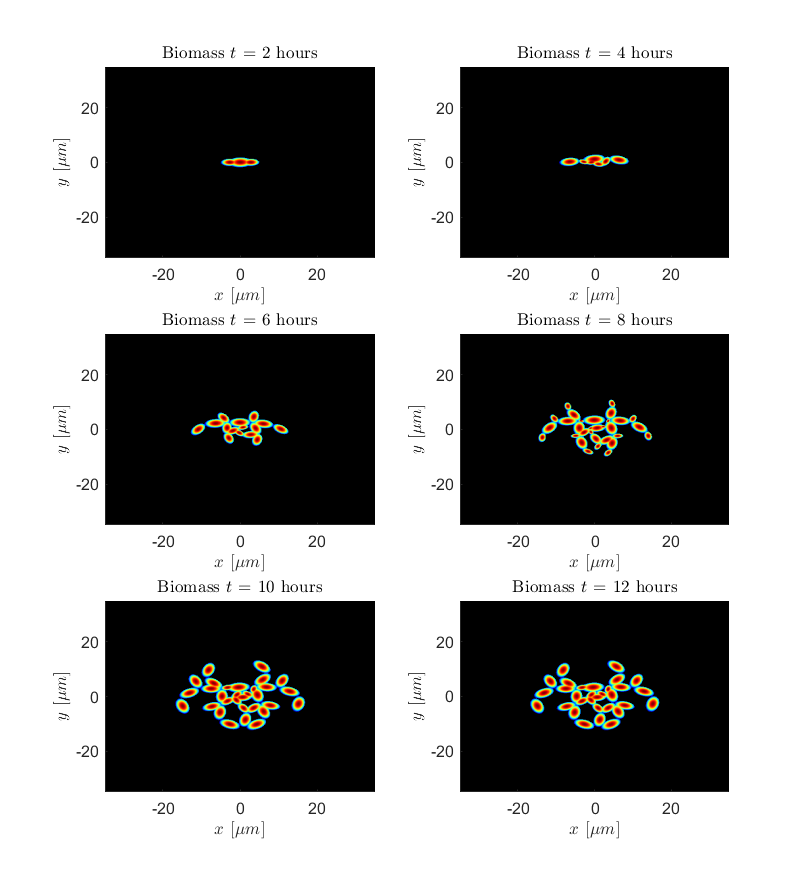
\includegraphics[width= 1\textwidth]{
        chapter2/figures/Biomass_t_all_L1_0o10_L2_1o00_L3_1o00_L4_1o00_L5_1o00_L6_3o00_L7_0o60.png}
    \caption{A cell colony with parameter values given by
             $\lambda_1 = 0.1$,  
             $\lambda_2 = 1.0$, 
             $\lambda_3 = 1.0$, 
             $\lambda_4 = 1.0$, 
             $\lambda_5 = 1.0$, 
             $\lambda_6 = 3.0$, 
             $\lambda_7 = 0.6$}
    \label{fig:ColonySimulationNutrientFieldN210}
    \end{figure}
    \filbreak


    \begin{figure}[h] %Change this to [p] maybe ?
        \centering
        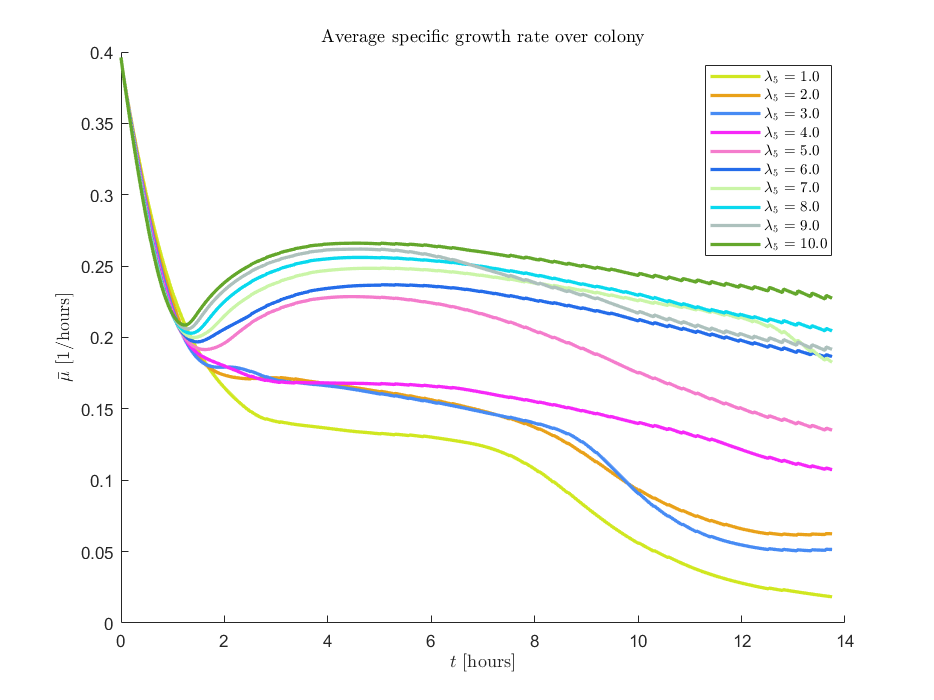
\includegraphics[width= 1\textwidth]{
            chapter2/figures/SpecificGrowthRatePlot.png}
        \caption{The colony average specific growth rate for different values of $\lambda_5$
                 is measured and plotted over time for ensemble size $1$. The rest of the parameters 
                 took the values:
                 $\lambda_1 = 0.1$,  
                 $\lambda_2 = 1.0$, 
                 $\lambda_3 = 1.0$, 
                 $\lambda_4 = 1.0$, 
                 $\lambda_5$ (variable), 
                 $\lambda_6 = 0.5$, 
                 $\lambda_7 = 0.7$.
                 Remarkably, when $\lambda_5 \geq 5.0$ there is an interesting dynamic that 
                 occurs based on the compettition between nutrient consumption rate ($\lambda_6$)
                 and the mobility ($\lambda_5$). For small values of mobility,
                 the cells are not able to move enough into areas where the nutrient has not 
                 decayed.}
        \label{fig:ColonySimulationNutrientFieldN210}
        \end{figure}
        \filbreak

\begin{figure}[h]
    \centering
    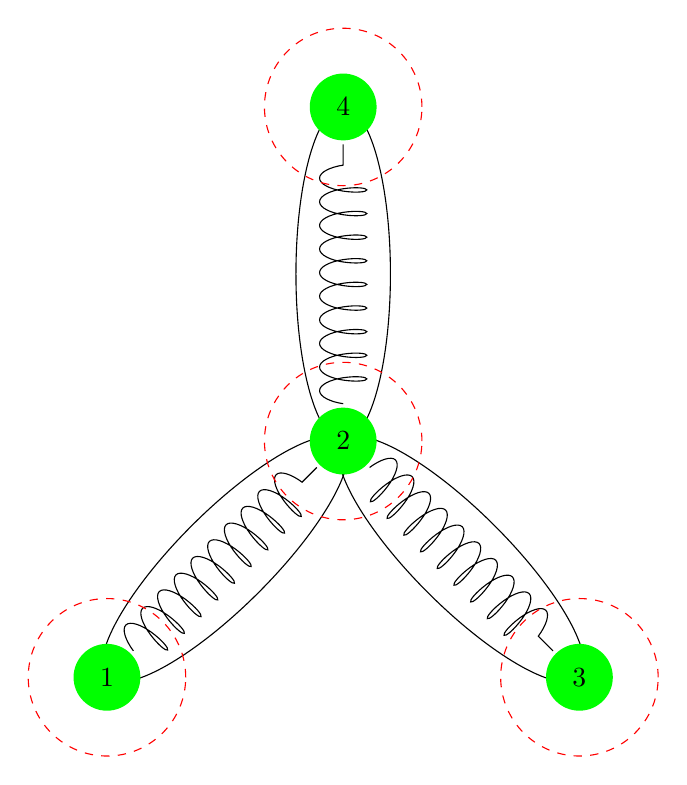
\begin{tikzpicture}
        \draw[rotate=45] (-0.5*4.243cm,0) ellipse (0.5*4.243cm and 0.6cm);
        \draw[rotate=-45] (0.5* 4.243,0) ellipse (0.5*4.243cm and 0.6cm);
        \draw[rotate=0] (0.0,0.5* 4.243)  ellipse (0.6cm and 0.5*4.243cm);
        
        \node[circle,fill=green, line width=1mm,inner sep=2.0mm] (a) at (-3,-3)  {1};
        \node[circle,fill=green, line width=1mm,inner sep=2.0mm] (b) at (0,  0)  {2};
        \node[circle,fill=green, line width=1mm,inner sep=2.0mm] (c) at (3, -3)  {3};
        \node[circle,fill=green, line width=1mm,inner sep=2.0mm] (d) at (0,4.243){4};
        \draw[decoration={aspect=0.3, segment length=3mm, amplitude=3mm,coil},decorate] (a) -- (b);
        \draw[decoration={aspect=0.3, segment length=3mm, amplitude=3mm,coil},decorate] (b) -- (c);  
        \draw[decoration={aspect=0.3, segment length=3mm, amplitude=3mm,coil},decorate] (b) -- (d); 

        \draw[dashed, color=red]   (a)  ellipse (1.0cm and 1.0cm);
        \draw[dashed, color=red]   (b)  ellipse (1.0cm and 1.0cm);
        \draw[dashed, color=red]   (c)  ellipse (1.0cm and 1.0cm);
        \draw[dashed, color=red]   (d)  ellipse (1.0cm and 1.0cm);
    \end{tikzpicture}
    \caption{A diagram of three elliptical cells with internal springs to represent biomass 
             elasticity ($\lambda_2 = \frac{K}{\eta \mu}$). The nodes are positioned at the ends of the major dimension
             of each ellipse and there are two nodes per cell. The force acting on 
             node $2$ for instance would be due to the forces from nodes $1$, $3$ and $4$.
             The dashed red circles represent the activation radius ($ \lambda_4 = R/L_0$) 
             of the contact force between the nodes.}
\end{figure}


\begin{figure}[h]
    \centering
    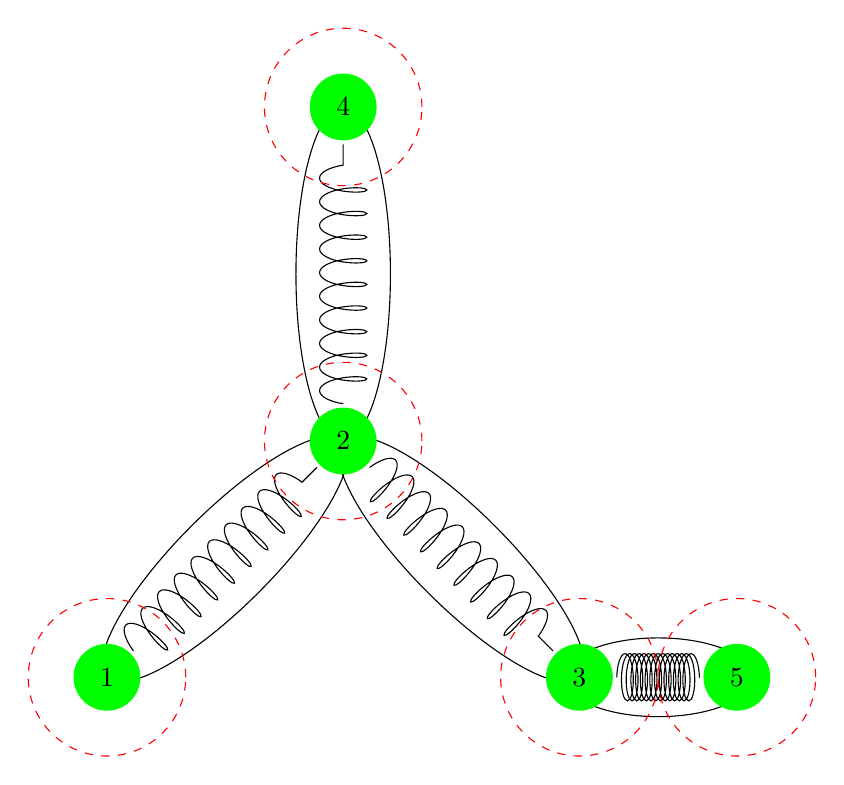
\begin{tikzpicture}
        \draw[rotate=45] (-0.5*4.243cm,0) ellipse (0.5*4.243cm and 0.6cm);
        \draw[rotate=-45] (0.5* 4.243,0) ellipse (0.5*4.243cm and 0.6cm);
        \draw[rotate=0] (0.0,0.5* 4.243)  ellipse (0.6cm and 0.5*4.243cm);
        \draw[rotate=0] (4.0,-3.0)  ellipse (1.2cm and 0.5cm);

        \node[circle,fill=green, line width=1mm,inner sep=2.0mm] (a) at (-3,-3)  {1};
        \node[circle,fill=green, line width=1mm,inner sep=2.0mm] (b) at (0,  0)  {2};
        \node[circle,fill=green, line width=1mm,inner sep=2.0mm] (c) at (3, -3)  {3};
        \node[circle,fill=green, line width=1mm,inner sep=2.0mm] (d) at (0,4.243){4};
        \node[circle,fill=green, line width=1mm,inner sep=2.0mm] (e) at (5,-3){5};
        \draw[decoration={aspect=0.3, segment length=3mm, amplitude=3mm,coil},decorate] (a) -- (b);
        \draw[decoration={aspect=0.3, segment length=3mm, amplitude=3mm,coil},decorate] (b) -- (c);  
        \draw[decoration={aspect=0.3, segment length=3mm, amplitude=3mm,coil},decorate] (b) -- (d); 
        \draw[decoration={aspect=0.3, segment length=0.6mm, amplitude=3mm,coil},decorate] (c) -- (e); 

        \draw[dashed, color=red]   (a)  ellipse (1.0cm and 1.0cm);
        \draw[dashed, color=red]   (b)  ellipse (1.0cm and 1.0cm);
        \draw[dashed, color=red]   (c)  ellipse (1.0cm and 1.0cm);
        \draw[dashed, color=red]   (d)  ellipse (1.0cm and 1.0cm);
        \draw[dashed, color=red]   (e)  ellipse (1.0cm and 1.0cm);
    \end{tikzpicture}
    \caption{A mitosis event occurs via the addition of new nodes connected to old nodes.
             The nodes are added very close (distance $\delta \ll 1$) by the original nodes (exaggerated here)
             so that the spring force can be defined. After this point, 
             the initially compressed cell ``grows" outwards to achieve its nominal length, under 
             the influence of elasticity, contact and chemotactic forces.}
\end{figure}











